\documentclass[12pt, a4paper, listof=totoc, bibliography=totoc, numbers=noenddot, ngerman, headsepline, oneside]{scrbook}
\usepackage{amsmath}
\usepackage[T1]{fontenc}
\usepackage{float}
\usepackage[utf8]{inputenc}
\usepackage[ngerman]{babel}
\usepackage{url}
\usepackage{graphicx} 
\usepackage{pdfpages} 
\usepackage[a4paper, margin=1in]{geometry}
\usepackage[right]{eurosym} %Euro-Zeichen
\usepackage{amssymb}
\usepackage{subfig}
\usepackage{cite} %Quellenangaben
\usepackage{setspace} % Zeilenabstand
\usepackage[ 
   colorlinks,       
   linkcolor=black,   % Farbe interner Verweise 
   filecolor=black,   % Farbe externer Verweise 
   citecolor=black,   % Farbe von Zitaten 
   urlcolor=blue	  % Farbe von Links
   ]{hyperref} %Verlinkungen
\usepackage[figure]{hypcap}
\usepackage[ngerman]{translator}
\usepackage{blindtext} % Lorem-Ipsum-Plugin
\usepackage{glossaries}

\usepackage{listings,xcolor} %Codeanzeige
\usepackage{scrhack}
\usepackage[normalem]{ulem}
\useunder{\uline}{\ul}{}
\usepackage{wrapfig}

\usepackage{makecell}
\usepackage{comment}
\renewcommand{\familydefault}{\sfdefault} %%SCHRIFTART
\usepackage{pifont}

\graphicspath{ {./bilder/} }


\usepackage{chngcntr}
\usepackage{color}
\counterwithout{figure}{chapter}
\counterwithout{table}{chapter}

\definecolor{dkgreen}{rgb}{0,.6,0}
\definecolor{dkblue}{rgb}{0.337, 0.612, 0.839}
\definecolor{dkyellow}{rgb}{204, 255, 0}
\definecolor{lila}{rgb}{0.847, 0.624, 0.855}
\definecolor{hintergrund}{rgb}{0.118, 0.118, 0.118}
\definecolor{blau1}{rgb}{0.573, 0.820, 0.925}
\definecolor{orange}{rgb}{0.839, 0.616, 0.522}
\definecolor{psrot}{rgb}{0.66, 0.18, 0.00}
\definecolor{psblau}{rgb}{0, 0, 0.545}
\definecolor{psbg}{rgb}{0.9176, 0.9490, 0.9804}
\definecolor{psbg2}{rgb}{0.949, 0.949, 0.949}
\definecolor{psbg3}{rgb}{1.0, 0.9843, 0.9608}



\lstset{
    numbers=left, 
    numberstyle=\tiny\color{black}, 
    numbersep=5pt,
    breaklines=true,
    frame=lr,
    escapeinside={(*@}{@*)}, %nicht anzuzeigende Ausdrücke, z.B. für Labels
    language=[Sharp]C,
    showstringspaces=false,
    captionpos=b,
    backgroundcolor=\color{hintergrund},
    basicstyle=\ttfamily\fontsize{9}{10}\selectfont\color{white},
    keywordstyle    = \color{dkblue},
    stringstyle     = \color{orange},
    identifierstyle = \color{blau1},
    commentstyle    = \color{dkyellow},
    emph            =[1]{var},
    emphstyle       =[1]\color{dkblue},
    emph            =[2]{if,and,or,else, return},
    emphstyle       =[2]\color{lila}
    ƒ} 
\lstdefinestyle{cli}{
    basicstyle=\ttfamily\fontsize{9}{10}\selectfont\color{white},
    identifierstyle = \color{white},
    numbers=none,
    language=sh,
    stringstyle=\color{dkblue},
    emph            =[1]{dotnet},
    emphstyle       =[1]\color{dkyellow},
}
\lstdefinestyle{tiny}{
    basicstyle=\ttfamily\fontsize{7}{8}\selectfont\color{white},
    numbers=left, 
    numberstyle=\tiny\color{black}, 
    numbersep=5pt,
    breaklines=true,
    frame=lr,
    escapeinside={(*@}{@*)}, %nicht anzuzeigende Ausdrücke, z.B. für Labels
    language=[Sharp]C,
    showstringspaces=false,
    captionpos=t,
    backgroundcolor=\color{hintergrund},
    keywordstyle    = \color{dkblue},
    stringstyle     = \color{orange},
    identifierstyle = \color{blau1},
    commentstyle    = \color{dkyellow},
    emph            =[1]{var},
    emphstyle       =[1]\color{dkblue},
    emph            =[2]{if,and,or,else, return},
    emphstyle       =[2]\color{lila}
}
\lstdefinestyle{ps}{
    numbers=left, 
    numberstyle=\tiny\color{black}, 
    numbersep=5pt,
    breaklines=true,
    frame=none,
    escapeinside={(*@}{@*)}, %nicht anzuzeigende Ausdrücke, z.B. für Labels
    language=sh,
    showstringspaces=false,
    captionpos=b,
    backgroundcolor=\color{psbg3},
    basicstyle=\ttfamily\fontsize{9}{10}\selectfont\color{black},
    keywordstyle    = \color{psblau},
    stringstyle     = \color{psrot},
    identifierstyle = \color{psrot},
    commentstyle    = \color{dkyellow},
    emph            =[1]{var},
    emphstyle       =[1]\color{dkblue},
    emph            =[2]{if,and,or,else, return},
    emphstyle       =[2]\color{lila}
}
    

\renewcommand\lstlistingname{Codeausschnitt}
\renewcommand\lstlistlistingname{Codeverzeichnis}

\geometry{verbose,tmargin=2cm,bmargin=2cm,lmargin=2cm,rmargin=2.3cm} 

\clubpenalty = 10000 \widowpenalty = 10000 \displaywidowpenalty = 10000 

\newcommand{\footfigref}[1]{\footnote{Abb. \ref{#1} auf Seite \pageref{#1}}}

%% Bei Referenzen im Text wird jetzt bei allen Ebenen "Kapitel" vorgestellt, z.b. Kapitel 2, Kapitel 2.2, Kapitel 6.3.2
\addto\extrasngerman{%
    \def\sectionautorefname{Kapitel}%
    \def\subsectionautorefname{Kapitel}%
    \def\subsubsectionautorefname{Kapitel}%
    }

% Vertikaler Abstand zwischen Ende Textblock - Ende Fußzeile --> Abstand der Seitenzahl von Rand erhöhen 
\setlength{\footskip}{10mm}

\RedeclareSectionCommand[%
    beforeskip=0.5\baselineskip,
    afterskip=0.5\baselineskip
]{chapter}

\RedeclareSectionCommand[%
    beforeskip=0.5\baselineskip,
    afterskip=0.5\baselineskip
]{section}

\RedeclareSectionCommand[%
    beforeskip=0.1\baselineskip,
    afterskip=0.1\baselineskip
]{subsection}

\RedeclareSectionCommand[%
    beforeskip=0.1\baselineskip,
    afterskip=0.1\baselineskip
]{subsubsection}

\RedeclareSectionCommand[%
    beforeskip=0.01\baselineskip,
    %%afterskip=0.2\baselineskip
]{paragraph}

\setlength{\abovecaptionskip}{4pt}  % 1pc=12pt 
\setlength{\belowcaptionskip}{0pt}
%\setlength{\textfloatsep}{4pt}
\setlength{\intextsep}{1pc}

%% Verkleinerung der Textgröße unter Abbildungen
\addtokomafont{caption}{\small}

%%falsche Default-Silbentrennung überschreiben
\hyphenation{Soft-ware-ent-wick-lung}


\renewcommand*{\glspostdescription}{}

%Glossar-Befehle anschalten
%\makeglossaries
 
\KOMAoptions{parskip=full*}

% ändert Titelschriftart in Serifen-Normalschriftart
\addtokomafont{disposition}{\rmfamily} 

\makenoidxglossaries

\loadglsentries{glossar.tex}

\newcommand{\type}{Software Engineering I - Paper}
\newcommand{\topic}{Grow Green}
\newcommand{\subtopic}{Ein Pixelart-Pflanzenpflege-Spiel}
\newcommand{\Alex}{Alexander Betke (77203378972)}
\newcommand{\Maja}{Maja Günther (72205653284)}
\newcommand{\Theo}{Theo Leuthardt (77205844868)}
\newcommand{\Josh}{Josh Nicolai Tischer (77207542779)}
\newcommand{\Domi}{Domenik Wilhelm (77207300494)}
\newcommand{\gruppe}{2}
\newcommand{\jahrgang}{2023}
\newcommand{\fachbereich}{Duales Studium Wirtschaft · Technik}
\newcommand{\studiengang}{Informatik}
\newcommand{\modul}{IT2101 - Software Engineering I}
\newcommand{\betreuerHS}{Benjamin Kretzmer}
\newcommand{\wordCount}{2800}


\begin{document}
\author{}

\title{
\normalfont\endgraf\rule{\textwidth}{1pt}
\begingroup
	\centering
	\linespread{1.5}
	\huge\topic
\endgroup
\linespread{1.5}
\ \\ % Falls kein Subtopic, auskommentieren
\large\subtopic % Falls kein Subtopic, auskommentieren
\normalfont\endgraf\rule{\textwidth}{1pt}
}

\date{\large vorgelegt am 05. November 2024}

\publishers{
	\begin{tabular}{l l}
    \textbf{\normalsize{}} & \normalsize{}  \tabularnewline
    \textbf{\normalsize{}} & \normalsize{}  \tabularnewline
	\textbf{\normalsize{Modul:}} & \normalsize{\modul}  \tabularnewline
    \textbf{\normalsize{Gruppe:}} & \normalsize{\gruppe}  \tabularnewline
	\textbf{\normalsize{Namen:}} & \normalsize{\Alex}  \tabularnewline
 	\textbf{\normalsize{}} & \normalsize{\Maja}  \tabularnewline
   	\textbf{\normalsize{}} & \normalsize{\Theo}  \tabularnewline
    \textbf{\normalsize{}} & \normalsize{\Josh}  \tabularnewline
    \textbf{\normalsize{}} & \normalsize{\Domi}  \tabularnewline
	\textbf{\normalsize{Studienjahrgang:}} & \normalsize{\jahrgang}  \tabularnewline
	\textbf{\normalsize{Fachbereich:}} & \normalsize{\fachbereich} \tabularnewline
	\textbf{\normalsize{Studiengang:}} & \normalsize{\studiengang} \tabularnewline
	\textbf{\normalsize{Betreuerin Hochschule:}} & \normalsize{\betreuerHS} \tabularnewline
    \textbf{\normalsize{Anzahl der Wörter:}} & \normalsize{\wordCount} \tabularnewline
    \tabularnewline
    \tabularnewline
	\end{tabular}
    \begin{tabular}{p{4.6em} p{0.3em} p{4.6em} p{0.3em} p{4.6em} p{0.3em} p{4.6em} p{0.3em} p{4.6em}}
        \hspace{4.5cm} && \hspace{4.5cm} && \hspace{4.5cm} && \hspace{4.5cm} && \hspace{4.5cm}\\
        \hspace{4.5cm} && \hspace{4.5cm} && \hspace{4.5cm} && \hspace{4.5cm} && \hspace{4.5cm}\\
        \cline{1-1}\cline{3-3}\cline{5-5}\cline{7-7}\cline{9-9} 
        \small{Alexander Betke} && \small{Maja Günther} && \small{Theo Leuthardt} && \small{Josh Tischer} && \small{Domenik Wilhelm}
    \end{tabular}
	}

\titlehead{\begin{center}
    
\includegraphics[height=0.031\textheight]{bilder/HWR.png}
    \hfill
    
\includegraphics[height=0.031\textheight]{bilder/Polizei.png}
    \hfill
    
\includegraphics[height=0.023\textheight]{bilder/FUBIT.png}
    \hfill
    
\includegraphics[height=0.026\textheight]{bilder/BDR.jpg}
    \hfill
    
\includegraphics[height=0.029\textheight]{bilder/Alstom.png}
    \end{center}
    }

\maketitle
\onehalfspacing 
\pagenumbering{Roman}
\chapter*{Abstract}
\addcontentsline{toc}{chapter}{Abstract}
das wird schon! \cite{FUB23}\\
\acrfull{FU}\\

\clearpage

\newpage

\tableofcontents{}
\addcontentsline{toc}{chapter}{Inhaltsverzeichnis}

\clearpage

\addcontentsline{toc}{chapter}{Akronyme}
\printnoidxglossary[type=\acronymtype]
\clearpage

\addcontentsline{toc}{chapter}{Glossar}
\printnoidxglossary
\clearpage

\chapter{Kurzbeschreibung}\label{ch:kurzbeschreibung}
\pagenumbering{arabic}
Pflanzen im Eigenheimoder Garten sorgen für ein natürliches Ambiente und ein geerdetes Umgebungsgefühl.\\
Doch nicht jeder hat die benötigten Gewohnheiten, um sich fachgerecht um seine Pflanzen zu kümmern.
GrowGreen soll dabei helfen, die Pflege von Pflanzen zu erleichtern und das Aneignen von Gewohnheiten 
zu einem spielerischen Erlebnis zu machen.\\[7pt]
% Was soll gemacht werden?
Ziel dieses Projekts ist es, eine Spielumgebung zu erschaffen, die Nutzern ermöglicht ihre realen Pflanzen auch virtuell zu besitzen 
und sich parallel in beiden Dimensionen bestmöglich um sie zu kümmern. 
Für Coins können eine begrenzte Auswahl der virtuellen Pflanzen gekauft werden, innerhalb des Shops. 
Pflegt der Spieler seine Pflanzen gut oder spielt in einem abgetrennten Modus Minispiele, verdient er damit Coins. 
Gut gepflegte Pflanzen ermöglichen den Spielern, ihren Wohnraum zu vergrößern. Die Spielfläche kann um ein
Gewächshaus erweitert werden.\\[7pt]
% Welche groben Zielen sollen verfolgt werden?
Zur Entwicklung von Gewohnheiten findet das Spiel in Echtzeit statt, so dass gleichzeitig auch die realen Pflanzen
außerhalb des Spiels wachsen und gedeihen.
Die virtuellen Pflanzen wachsen auch in Echtzeit und müssen regelmäßig gegossen und gepflegt werden.
Die Gießintervalle und Wachstumsphasen sind authentisch festgelegt.
Während Spieler diese Intervalle abwarten, können sie beispielweise Minispiele spielen, um die Zeit zu verbringen und 
Münzen zu verdienen. \\[7pt]
% Welchen Nutzen/Mehrwert bringt die Lösung für die Gesellschaft?
GrowGreen ist ein abwechslungsreiches Spiel für Pflanzenliebhaber, vor allem diese, die Schwierigkeiten bei der Wartung und 
Pflege ihrer Topfpflanzen haben. Die direkte Zielgruppe sind damit neurodiverse, vielbeschäftigte oder auch einfach vergessliche Personen. Wer von einen eigenen Garten träumt, ist hier genau richtig. 
Das Projekt erleichtert Nutzern Verantwortung für Lebewesen zu übernehmen und sich Wissen zu ihren Pflanzen 
spielerisch anzueignen. So werden nachhaltig Gewohnheiten zur der Pflanzenpflege entwickelt.\\[7pt]
% Wie ist die Vision?
Unser 2D Pixelart Spiel soll ein Verständnis für die Bedürfnisse und Ansprüche von gängigen Topfflanzen erwecken.
Zusätzlich zur Gewohnheitsbildung soll das Spiel einen Spaßfaktor bieten, um die langfristige Nutzung zu garantieren.
In ferner Zukunft ist eine Zusammenarbeit mit Blumenläden und Baumärkten in Ausblick, um
das verfügbare Repertoire an Pflanzen, Blumen und Gartenzubehör zu erweitern. \\[7pt]
% Wann ist das Projekt ein Erfolg?
Wir sehen GrowGreen als volen Erfolg an, da eine spielbare Version mit allen grundlegend benötigten Hauptkomponenten 
erstellt und veröffentlicht wurde.
Dabei werden Spielerdaten gespeichert und können später wieder aufgerufen werden.
Bestenfalls wird das Projekt gut aufgenommen und für Begeisterung in der Bevölkerung sorgen.
\chapter{Projektsteckbrief}\label{ch:steckbrief}

\chapter{Ziele}\label{ch:ziele}
\begin{table}[]
    \centering
    \begin{tabular}{ccccc}
        \hline
        \multicolumn{1}{|c|}{\textbf{Nr.}} & \multicolumn{1}{c|}{\textbf{Klassifizierung}} & \multicolumn{1}{c|}{\textbf{Beschreibung}}                                                                                                                        & \multicolumn{1}{c|}{\textbf{Messkriterium}}                                                                                                                                                                  & \multicolumn{1}{c|}{\textbf{Priorität}} \\ \hline
        1                                  & Leistung                                      & Hauptszene                                                                                                                                                        & \begin{tabular}[c]{@{}c@{}}Hintergrund und Logik zu Spielerbewegung sowie\\ Pflanzenplazierlogik wurde implementiert.\end{tabular}                                                                           & Muss                                    \\
        2                                  & Leistung                                      & Titelmenü (Startmenü des Spiels)                                                                                                                                  & \begin{tabular}[c]{@{}c@{}}Zugehörige Menüpunkte zum Starten, Laden eines \\ Spiels, zur Charakterauswahl und zu den Einstellungen \\ wurden erstellt, dessen Logik implementiert und getestet.\end{tabular} & Muss                                    \\
        3                                  & Leistung                                      & Shopszene                                                                                                                                                         & \begin{tabular}[c]{@{}c@{}}Logik zum Kaufen und Verkaufen von Pflanzen, Kauf von\\ Pflanzensamen und Shopinterface wurde implementiert \\ und getestet.\end{tabular}                                         & Muss                                    \\
        4                                  & Leistung                                      & Weltszene                                                                                                                                                         & \begin{tabular}[c]{@{}c@{}}Szene sammt Szenenwechsellogik und -animation wurde \\ implementiert und getestet.\end{tabular}                                                                                   & Kann                                    \\
        5                                  & Leistung                                      & \begin{tabular}[c]{@{}c@{}}Implementierung der Pflanzenlogik bezüglich\\ Bewässerung und Pflanzenwachstum\end{tabular}                                            & \begin{tabular}[c]{@{}c@{}}Realistische Funktionalität wurde nach der Implementierung\\ getestet.\end{tabular}                                                                                               & Muss                                    \\
        6                                  & Leistung                                      & \begin{tabular}[c]{@{}c@{}}Backend in Form einer Datenbank \\ zur Speicherung aller Spieler- und Pflanzendaten\end{tabular}                                       & \begin{tabular}[c]{@{}c@{}}Spieler und Pflanzendaten werden korrekt gespeichert und \\ ausgelesen, Debuggingtools dienen zum Testen der Werte.\end{tabular}                                                  & Muss                                    \\
        7                                  & Leistung                                      & \begin{tabular}[c]{@{}c@{}}Bereitstellung von Github Actions zum automatisierten \\ Kompilieren des Papers sowie des Spiels \\ als ausführbare Datei\end{tabular} & \begin{tabular}[c]{@{}c@{}}Testweises Kompilieren der aktuellen Stände von Paper\\ und Spielprojekt auf Github\end{tabular}                                                                                  & Muss                                    \\
        8                                  & Leistung                                      & \begin{tabular}[c]{@{}c@{}}Texturen für Pflanzen, Töpfe und\\ weitere Assets des Spiels\end{tabular}                                                              & \begin{tabular}[c]{@{}c@{}}Speicherung aller benötigten Assets auf Github mit \\ entsprechender Verfügbarkeit in der Spielengine\end{tabular}                                                                & Muss                                    \\
        9                                  & Leistung                                      & Logoerstellung                                                                                                                                                    & \begin{tabular}[c]{@{}c@{}}Nutzung eines fertigen Logos in allen Facetten des Spiel\\ mit der Zufriedenheit aller Gruppenmitglieder\end{tabular}                                                             & Soll                                    \\
        10                                 & Hauptziel                                     & Fertigstellung des Papers                                                                                                                                         & \begin{tabular}[c]{@{}c@{}}Alle Kapitel wurden fertig gestellt mit zusätzlicher \\ Unterzeichnung der ehrenwörtlichen Erklärung aller\\ Gruppenmitglieder.\end{tabular}                                      & Muss                                    \\
        11                                 & Termin                                        & Fertigstellung der Spieleentwicklung                                                                                                                              & \begin{tabular}[c]{@{}c@{}}Das Spiel wird am 29.10.2024 um 23:59 Uhr fertig\\ gestellt in seiner Entwicklung.\end{tabular}                                                                                   & Kann                                    \\
        12                                 & Termin                                        & Endpräsentation                                                                                                                                                   & \begin{tabular}[c]{@{}c@{}}Vorstellung des Projekts bei der Endpräsentation mit \\ zusätzlicher Abgabe der Folien bei Moodle \\ bis zum 29.10.2024 um 23:59 Uhr\end{tabular}                                 & Muss                                    \\
        13                                 & Termin                                        & Abschluss des Projektes                                                                                                                                           & \begin{tabular}[c]{@{}c@{}}Pünktliche Abgabe des Source-Codes und der \\ Endpäsentation auf Moodle am 29.10.2024 \\ um 23:59 Uhr und des Papers am 05.11.2024 \\ um 23:59 Uhr\end{tabular}                   & Soll                                    \\
        14                                 & Leistung                                      & Sehr gute Bewertung des Projekts                                                                                                                                  & Gewünschte Bewertung vom Stakeholder wird erreicht                                                                                                                                                           & Soll                                    \\
        15                                 & Leistung                                      & \begin{tabular}[c]{@{}c@{}}Lerneffekt bei Nutzern des Spiels zum Wissen über\\ Pflanzen und Ökosysteme\end{tabular}                                               & Feedback von Nutzern des Spiels                                                                                                                                                                              & Soll                                    \\
        16                                 & Sozial                                        & \begin{tabular}[c]{@{}c@{}}Entwicklung von Gewohnheiten bei der Pflanzenpflege\\ der Haus- oder Gartenpflanzen des Nutzers\end{tabular}                           & Feedback von Nutzern des Spiels                                                                                                                                                                              & Soll                                    \\
        17                                 & Leistung                                      & Nutzer haben Spaß am Spielen von Grow Green                                                                                                                       & Feedback von Nutzern des Spiels                                                                                                                                                                              & Kann
    \end{tabular}\label{tab:projektziele}
\end{table}
\chapter{Aufgaben - Kompetenzen - Verantwortlichkeiten (AKV)}\label{ch:AKV}
Um komplikationsfrei das Projekt durchführen zu können, ist es ein essentieller Schritt innerhalb
des Teams jedem Gruppenmitglied eine oder mehrere Rollen zuzuweisen.
Damit sämtliche Erfahrungen und Fähigkeiten aller Gruppenmitglieder optimal genutzt werden können, 
ist es wichtig die Rollen so zu verteilen, dass jeder seine Stärken einbringen kann. 
Dies trägt dazu bei die Zeit in den Arbeitszeitblöcken effizient zu nutzen, indem keine der aktuellen Aufgaben
mehrfach bearbeitet werden. 
Demnach ergibt sich folgende Rollenverteilung, die innerhalb der folgenden AKV-Matrizen näher erläutert wird.

\vspace{1cm}
\begin{table}[H]
    \begin{center}
        \label{tab:projektmanager}
        \begin{tabular}{|c||p{9cm}|}
            \hline
            Aufgaben & Kontrolle aller tabellarischen Dokumente sowie des \\
            & Zeitmanagements inklusive Einhaltung der Fristen, \\
            & Dokumentation der Aufwandsschätzung und des\\
            & Risikomanagements, Qualitätskontrolle der Software \\
            & und Management des Entwicklungsablaufs \\
            \hline
            Kompetenzen & Erstellung der Tabellen (Excelkenntnisse), \\
            & Erinnerung anderer Gruppenmitglieder an Fristen, \\
            & Qualitätskriterien beachten bei der Entwicklung, \\
            & Aufwände präsent halten \\
            \hline
            Verantwortlichkeiten & Korrekten Verlauf des Projekts sicherstellen, \\
            & Einhaltung von Fristen, regelmäßiges Prüfen aller  \\
            & Dokumentationen und Managementtabellen \\
            \hline
        \end{tabular}
        \caption{AKV-Matrix des Projektmanagers}
    \end{center}
\end{table}
\begin{table}[H]
    \begin{center}
        \label{tab:devopsengineer}
        \begin{tabular}{|c||p{9cm}|}
            \hline
            Aufgaben & Implementierung von Github Actions über YAML- \\
            & Dateien mit entsprechender Erstellung von \\
            & Automatisierungsmechanismen des Kompilierungs- \\ 
            & vorgangs von Projekt und Paper, Testung der\\
            & implementierten Actions mit anschließender \\
            & Überprüfung der erstellten Binärdateien und der \\
            & korrekten Erstellung von Github Releases \\
            \hline
            Kompetenzen & Erstellen von Github Actions und Workflows,  \\
            & Verstehen des Syntax von Workflow YAML-Dateien, \\
            & Debugging von fehlgeschlagenen Testbuilds \\
            \hline
            Verantwortlichkeiten & Infrastruktur zur Kompilierung des Projekts und \\
            & des Papers zur automatisierten Bereitstellung von \\
            & PDF- und Binärdateien \\
            \hline
        \end{tabular}
        \caption{AKV-Matrix des Dev-Ops-Engineers}
    \end{center}
\end{table}
\begin{table}[H]
    \begin{center}
        \label{tab:softwareentwickler}
        \begin{tabular}{|c||p{9cm}|}
            \hline
            Aufgaben & Entwicklung der definierten Features in GODOT, \\
            & Schreiben von Skripten in C\# und SQL mit \\
            & anschließender Pull-Request von der eigenen \\
            & zur main-Branch, Benutzung von erstellten Assets\\
            & für Engine-spezifische Objekte, Einbindung von \\
            & Shadern und Animationen, Reviewen und Testen des Code \\
            \hline
            Kompetenzen & Erstellung und Bearbeitung sowie sicherer Umgang \\
            & mit Branches und Pull-Requests auf Github, selbst- \\
            & ständiges Management des Kanbansystems auf \\
            & Github, Spieleentwicklung mit der GODOT- \\
            & Engine, Überprüfung von Code in Pull-Request \\
            \hline
            Verantwortlichkeiten & Funktionierende Implementierung der Features \\
            & mit Bug-Fixing, Einhaltung der Frist für die \\
            & Entwicklung des Spiels, Gewährleistung von \\
            & Codequalität \\
            \hline
        \end{tabular}
        \caption{AKV-Matrix des Softwareentwicklers}
    \end{center}
\end{table}
\begin{table}[H]
    \begin{center}
        \label{tab:paperautor}
        \begin{tabular}{|c||p{9cm}|}
            \hline
            Aufgaben & Verfassen von Texten und Tabellen für das Paper, \\
            & Korrekturarbeit bei den von anderen Paperautoren \\
            & geschriebenen Kapiteln oder Texten \\
            \hline
            Kompetenzen & Umgang mit LaTeX und Tabellen im LaTeX-Format, \\
            & Verwaltung des Paperversionierung auf Github über \\
            & Branches und Pull-Requests \\
            \hline
            Verantwortlichkeiten & Fristgemäße Fertigstellung des Papers in korrekter \\
            & deutscher Rechtschreibung und Grammatik, \\
            & Formatierung des Papers \\
            \hline
        \end{tabular}
        \caption{AKV-Matrix des Paperautors}
    \end{center}
\end{table}
\begin{table}[H]
    \begin{center}
        \label{tab:designer}
        \begin{tabular}{|c||p{9cm}|}
            \hline
            Aufgaben & Entwerfen und Zeichnen der Assets für Spieltexturen \\
            & wie Pflanzen, Töpfe, Hintergründe, Button-Icons und \\
            & und Objektrahmen, Sammeln von Pflanzenarten für die Datenbank \\
            \hline
            Kompetenzen & Erstellung von Assets für Texturen mit Pixelart- \\
            & Tool, Hochladen der Assets auf Github in den \\
            & Projektordner, Recherche zu Pflanzen, \\
            & Höchstmaß an Kreativität \\
            \hline
            Verantwortlichkeiten & Bereitstellung von Assets für Texturen zur nahtlosen \\
            & Entwicklung des Spiels und Pflanzenfakten zur \\
            & Speicherung in der Datenbank \\
            \hline
        \end{tabular}
        \caption{AKV-Matrix des Designers}
    \end{center}
\end{table}

\vspace{5cm}

Mit den zuvor beschrieben Rollen werden alle Aufgaben im Projekt Grow Green abgedeckt und
den jeweiligen Gruppenmitgliedern zugeordnet. 
Die Zuordnung wird nach Vorwissen, Erfahrungen, Interessen und Fähigkeiten getroffen. 
Die folgenden zwei Rollen werden besonders achtsam zugeteilt, da sie den Kern der Entwicklung des Spiels darstellen.
So wurden Gruppenmitgliedern die Rolle des Softwareentwicklers zugeordnet, falls diese sowohl Interesse
an der Programmierung und Erstellung des Spiels haben, als auch Erfahrungen mit der 
objektorientierten Programmierung.
Die Rolle des Designers wird nur denjenigen zugeordnet, die das höchste Maß an Kreativität der Gruppe besitzen
zum Erzielen der bestmöglichen Texturen des Spiels.
In folgender Matrix wird die Rollenverteilung des Grow Green-Teams dargestellt.

\vspace{2cm}

\begin{table}[H]
    \begin{center}
        \label{tab:rollenverteilung}
        \begin{tabular}{|c|c|c|c|c|c|}
            \hline
            Rollen 
            & Alexander 
            & Maja 
            & Theo 
            & Josh 
            & Domenik \\
            & Betke
            & Günther
            & Leuthardt
            & Tischer
            & Wilhelm \\
            \hline
            \hline
            Projektmanager &  &  &  &  & x \\
            \hline
            Dev-Ops-Engineer & x &  &  &  &  \\
            \hline
            Softwareentwickler &  &  &  & x &  \\
            \hline
            Paperautor &  &  & x &  &  \\
            \hline
            Designer &  & x &  &  &  \\
            \hline
        \end{tabular}
        \caption{Matrix zur Rollenverteilung}
    \end{center}
\end{table}
\chapter{Risikomanagement}\label{sec:risikomanagement}
\chapter{Aufwand}\label{ch:aufwand}
Zu Beginn des Projekts wird der zu nvestierende Aufwand geschätzt.
Die Schätzung erfolgt durch alle Teammitglieder und wird in Stunden gemessen.
So kann einerseits die Arbeitseffizienz beurteilt werden und andererseits der Fortschritt des Projekts.
Jeder Aufwand wird von einem oder mehreren Gruppenmitgliedern geschätzt, die für die Aufgabe zuständig sind und 
die höchste Expertise im jeweiligen Bereich haben. 
Die Schätzung wird in Stunden angegeben und in einer Tabelle festgehalten.\\
\newline
Unter anderem wird der Aufwand die Konzeptionierung und Realisierung des Spiels geschätzt.
Darin kommen Aufwände auf, wie die Ideenfindung oder die Erstellung des Produktstrukturplans 
(s. ~\autoref{fig:produktstrukturplan}) und das Erstellen des Risikomanagements in ~\autoref{ch:risikomanagement}.
Zur Realisierung gehören unter anderem die Programmierung des Spiels und die Dokumentation auf Entwickler-
beziehungsweise Anwenderebene, welche unser Kanban auf Github und die Anleitung zur Verwendung des Spiels in ~\autoref{ch:anleitung}.\\
\newline
Besonders hoch werden die Aufwände für die Realisierung insgesamt und die Meetings innerhalb der Gruppe geschätzt.
Die Realisierung wird zu Anfang des Projekts auf 154 Stunden geschätzt, da die Programmierung des Spiels eine große Hürde
durch das Aneignen von Programmierkenntnissen in der verwendeten Programmiersprache und Engine darstellt.
Zusätzlich werden die Meetings auf insgesamt 48 Stunden geschätzt, weil einerseits gemeinsame Entwicklungssitzungen dazu
beitragen zeiteffizienter zu programmieren, jedoch auch zeitlichen Aufwand darstellen gewonnen Erkenntnisse in der
Gruppe zu teilen.
Dazu kommt es in einer Gruppe von fünf Personen zu häufigeren Meinungsverschiedenheiten, die Diskussionen und damit
zeitaufwändigere Meetings zur Folge haben.
Als weiterer größter Aufwand werden Teile des Spiels bewertet, die als Risiko eingestuft wurden und somit auf der einen 
Seite sehr viel Zeit in Anspruch nehmen könnten oder mit dem Ende des Projekts nicht vollständig bis gar nicht umgesetzt
werden. \\
\newline
In folgender Tabelle wird die Aufwandsschätzung dargestellt mit den Daten, um welchen Aufwand es sich handelt und der
Personenzuweisung, der Schätzung in Stunden, dem Realaufwand in Stunden und der Differenz zwischen Schätzung und
Realaufwand.
Das Vorzeichen der Differenz gibt Auskunft darüber, ob sich über- oder unterschätzt wurde.
Dabei ist ein positives Vorzeichen eine Überschätzung und ein negatives Vorzeichen eine Unterschätzung.\\
\newpage
% Tabelle hier so:
\begin{table}[H]\label{tab:aufwand}
    \footnotesize
    \centering
    \begin{tabular}{|l|c|c|c|c|}
        \hline
        Position & Verantwortlicher & Schätzung & Real & Abweichung \\[0.5ex]
        \hline\hline
        \textbf{Konzeptionierung} & & \textbf{36} & \textbf{38} & \textbf{2} \\
        \hline
        Ideenfindung & 1,2,3,4,5 & 2 & 4 & 2 \\
        Produktstrukturplan & 1,2,3,4,5 & 3 & 3 & 0 \\
        Produktstruktur Flussplan & 1,2,3,4,5 & 1 & 1 & 0 \\
        Risikomanagement & 1,2,3,4,5 & 6 & 8 & 2 \\
        Skills aneignen & 1,2,3,4,5 & 24 & 22 & -2 \\[0.5ex]
        \hline\hline
        \textbf{Realisierung} & & \textbf{269} & \textbf{227,5} & \textbf{-46,5} \\
        \hline
        Dokumentation (Paper) & 2,3 & 40 & 47 & 7 \\
        Anwenderdoku (Anleitung) & 3 & 2 & 0,5 & -1,5 \\
        Entwicklerdoku (Kanban) & 1,5 & 7 & 5 & -2 \\
        Programmierung & 1,3,4,5 & 200 & 150 & -50 \\
        Design der Pflanzenassets & 2 & 10 & 10 & 0 \\
        Design weiterer Grafiken & 2 & 10 & 15 & 5 \\[0.5ex]
        \hline\hline
        \textbf{Test und Qualitätssicherung} & & \textbf{19} & \textbf{16} & \textbf{-3} \\
        \hline
        Entwicklertest & 1,3,4,5 & 15 & 13 & -2 \\
        Performancetest & 1,3 & 4 & 3 & -1 \\[0.5ex]
        \hline\hline
        \textbf{Go-Live} & & \textbf{10,5} & \textbf{7,5} & \textbf{-3} \\
        \hline
        Deployment & 1,3 & 10 & 7 & -3 \\
        Admin Einweisung & 1,3 & 0,5 & 0,5 & 0 \\[0.5ex]
        \hline\hline
        \textbf{Meetings} & & \textbf{45} & \textbf{35} & \textbf{-10} \\
        \hline
        Meetings zu fünft & 1,2,3,4,5 & 15 & 10 & -5 \\
        Hilfe untereinander & 1,2,3,4,5 & 30 & 25 & -5 \\[0.5ex]
        \hline\hline
        \textbf{Projektmanagement} & & \textbf{10} & \textbf{15} & \textbf{5} \\
        \hline
        Konkretisierung der Idee & 1,2,3,4,5 & 5 & 10 & 5 \\
        Kontrolle und Wartung der Tabellen & 5 & 5 & 5 & 0 \\[0.5ex]
        \hline\hline
        \textbf{Risiko} & & \textbf{40} & \textbf{20} & \textbf{-20} \\
        \hline
        Minispiele & 1,4,5 & 30 & 15 & -15 \\
        Pflanzenvielfalt & 2 & 10 & 5 & -5 \\[0.5ex]
        \hline\hline
        \textbf{Gesamt} & & \textbf{429,5} & \textbf{359} & \textbf{70,5} \\
        \hline
    \end{tabular}
    \caption{Aufwandsschätzung}
\end{table}
In der Realität haben wir uns bei unseren Aufwänden in allen Bereichen überschätzt, also wir mussten weniger
Zeitaufwand investieren als ursprünglich geschätzt. 
Von der Sicht des Projektstarts ist das aber plausibel, denn die vorhandenen Herausforderungen aus ~\autoref{ch:herausforderungen} bezüglich der Programmierung und Aneignung von Kenntnissen zu Engine und Programmiersprache
wirkten zeitaufwändiger als sie eigentlich waren.
Ebenfalls wurde der Workload von der Erstellung des Papers überschätzt, da sich die Erarbeitung durch Arbeitsteilung 
als weniger aufwändig herausstellte die Menge der Texte einen kleineren Anteil des Papers darstellte als die Tabellen.
Implementierungen wie die Minispiele oder das Erstellen vieler Pflanzenassets für eine erhöhte Pflanzenvielfalt wurden 
als Risiken eingestuft und somit als aufwändiger angenommen, als sie in der Realität waren. 
Zur Risikobehandlung wurde die Minispielanzahl reduziert und nicht wie anfangs gedacht zum Beispiel auf 5 
festgelegt für mehr Spielvarietät, was den Aufwand und das Risiko erheblich reduzierte.
Die Pflanzenassets wurden durch den Designer erweitert, was durch die Einarbeitung im Pixelart-Editor 
nicht die erwartete Aufwandshöhe erreichte und damit genauso das Risiko minderte.\\ 
\chapter{Produktstruktur}\label{ch:produktstruktur}
Der Produktstrukturplan ist eine grafische Darstellung der Struktur unseres Produktes und ist wichtig
zur Aufteilung des Produkts in seine einzelnen Bestandteile und Teilkomponenten.
Sobald initial die Struktur des Produktes festgelegt wird, kann auf dieser Basis der Aufwand für jede Teilkomponente des
Produkts geschätzt werden, wodurch summiert der Gesamtaufwand für das Projekt berechnet wird. 
Zusätzlich können betroffene Elemente in das Risikoregister eingetragen werden, falls bei Besprechungen innerhalb des 
Teams Bedenken aufkommen bezüglich der benötigten Zeit für die Umsetzung.
Außerdem kann der Produktstrukturplan Grundlage sein für die Ermittlung der Qualitätskriterien für die einzelnen 
Teilkomponenten des Produkts. 
In Abbildung ~\ref{fig:produktstrukturplan} ist der Produktstrukturplan für unser Projekt dargestellt.
\vspace{2cm}
\begin{figure}[h]
    \centering
    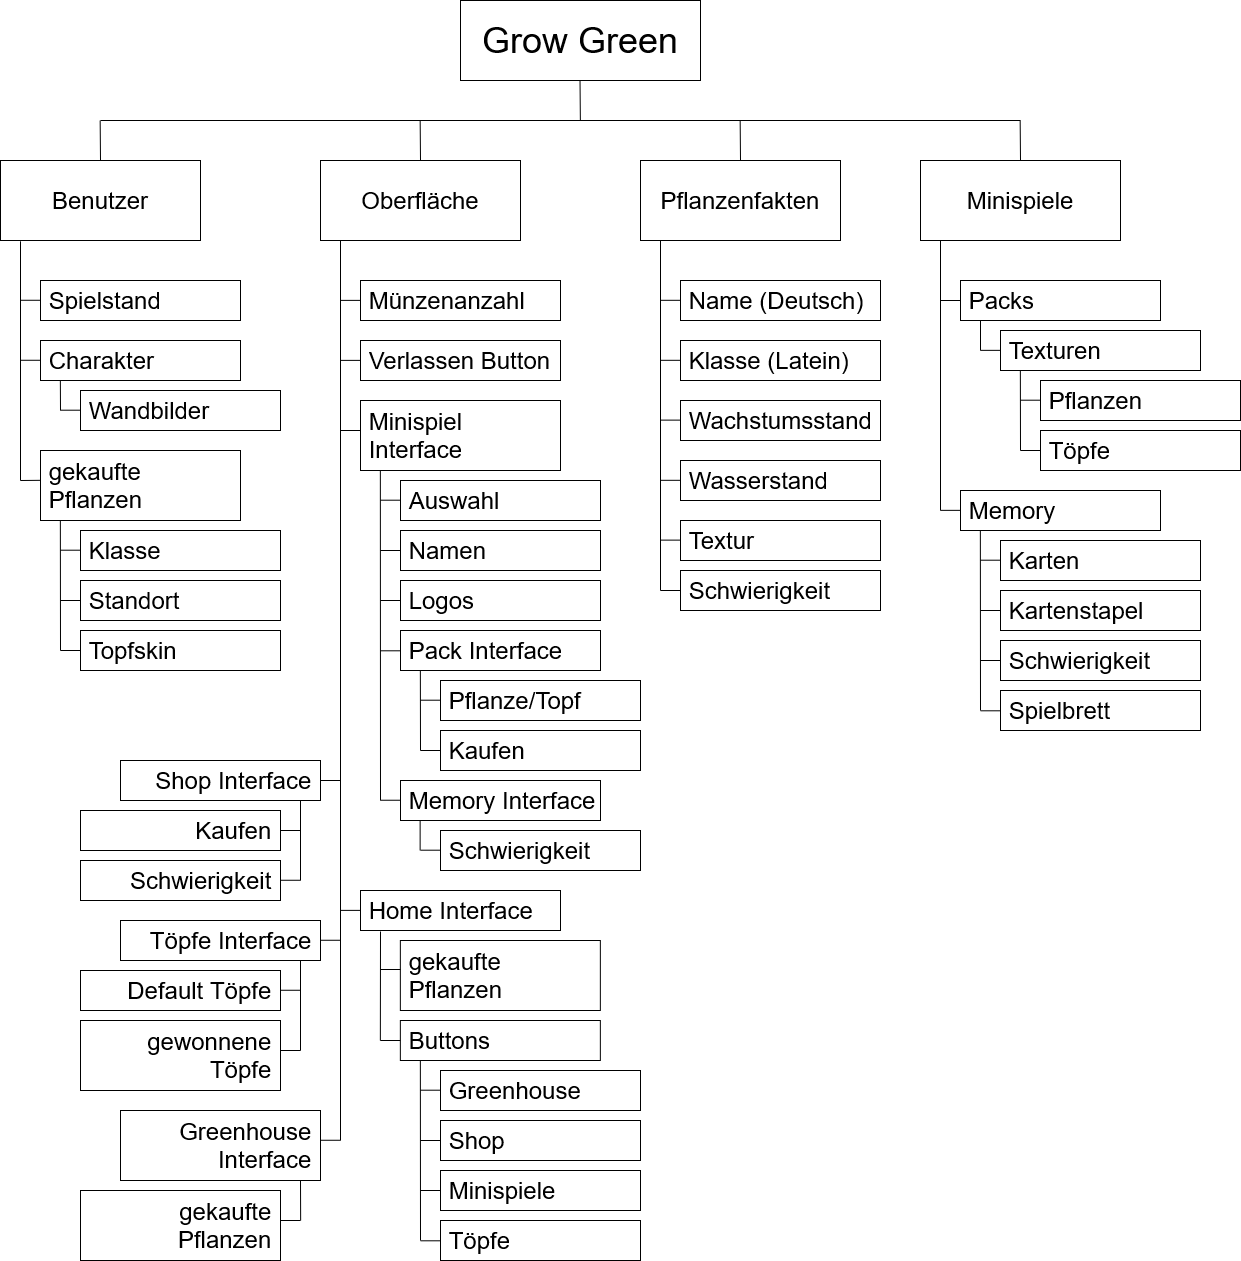
\includegraphics[width=\linewidth]{bilder/Produktstrukturplan.png}
    \caption{Produktstrukturplan}
    \label{fig:produktstrukturplan}
\end{figure}
\include{kapitel/08herausforderungen_lösungen}
\chapter{UML}\label{sec:uml}
\include{kapitel/10qualitätskriterien}
\chapter{Technologien und Produkte}\label{sec:technologien}
\chapter{Anleitung zur Verwendung}\label{ch:anleitung}
GrowGreen als ausführbare Datei ist über das GitHub Repository oder die Datei in der Moodle Abgabe erhältlich. 
Unter dem Tab „Releases“ wird in GitHub immer die aktuellste Version des Spiels veröffentlicht. Verfügbar für alle Betriebssysteme ist es dort als 
ZIP-Datei zu finden. 
Diese muss heruntergeladen und an einem beliebigen, gut erreichbaren Speicherort entpackt werden. 
Das Spiel wird gestartetdurch Ausführen der .exe Datei im eben extrahierten Ordner.\\
\newline
Zu Beginn des Spiels kann ein Charakter gewählt werden. 
Diese Wahl beeinflusst die Einrichtung der Spielumgebung. 
Wird ein neues Spiel erstellt, werden bereits existierende, alte Speicherstände überschrieben und ein neuer angelegt.\\
\newline
Über den Shop können nun die ersten Pflanzen gekauft werden. 
Nach dem Kauf einer Pflanze wird diese automatisch auf einem freien Platz im Haus platziert. 
Standardmäßig haben alle Pflanzen einen brauen Terrakotta-Topf. Die Farbe kann über das Töpfe-Menü mit dem Rucksack-Icon 
geändert werden. 
Dazu muss einfach ein Topf ausgewählt und dann, durch Klicken, auf eine Pflanze angewendet werden. 
Jede Topffarbe kann beliebig oft verwendet und die Farbe eines Topfes beliebig oft verändert werden. 
Platzierte Pflanzen können durch längeres Klicken verschoben und durch Verschieben in den Mülleimer, 
gelöscht werden.\\
\newline
Das Minigame-Menü bietet drei Auswahlmöglichkeiten. 
Aus den Plant-Packs lassen sich neue Pflanzen zu unschlagbaren Preisen gewinnen. 
Pot-Packs schalten dagegen neue, einzigartige Spezialtöpfe frei, die auf vorhandene Pflanzen angewendet werden können. 
Durch Spielen des Memory-Minispiels, können außerdem weitere Münzen verdient werden, die dann beispielsweise im Shop benutzt 
werden können.\\
\newline
Im anfänglichen Spielbereich befindet sich außerdem eine Tür in der Mitte. 
Diese kann für 100 Münzen geöffnet werden und schaltet den Zugang zum Greenhouse frei. 
Dieses funktioniert wie das Haupthaus und bietet dem Spieler mehr Platz, um Pflanzen unterzubringen.\\


\clearpage
\pagenumbering{Alph}

\bibliography{literatur}

\bibliographystyle{hwrbib}


\listoffigures
\lstlistoflistings

\listoftables
\addchap{Anhang}


\chapter*{Ehrenwörtliche Erklärungen}
\addcontentsline{toc}{chapter}{Ehrenwörtliche Erklärung}


Wir erklären ehrenwörtlich:
\begin{enumerate}
	\item dass wir unser Paper selbstständig verfasst habe,
	\item dass wir die Übernahme wörtlicher Zitate aus der Literatur sowie die Verwendung der Gedanken anderer Autoren an den entsprechenden Stellen innerhalb der Arbeit gekennzeichnet habe,
	\item dass wir unser Paper bei keiner anderen Prüfung vorgelegt haben.
\end{enumerate}
Wir sind uns bewusst, dass eine falsche Erklärung rechtliche Folgen haben wird.\\
\\ \\
\begin{tabular}{lp{2em}l} 
 \hspace{4cm}   && \hspace{7cm} \\\cline{1-1}\cline{3-3} 
 \small{Ort, Datum} && \small{Alexander Betke} \\
 \\\\
 \hspace{4cm}   && \hspace{7cm} \\\cline{1-1}\cline{3-3} 
 \small{Ort, Datum} && \small{Maja Günther} \\
 \\\\
  \hspace{4cm}   && \hspace{7cm} \\\cline{1-1}\cline{3-3} 
 \small{Ort, Datum} && \small{Theo Leuthardt} \\
 \\\\
  \hspace{4cm}   && \hspace{7cm} \\\cline{1-1}\cline{3-3} 
 \small{Ort, Datum} && \small{Josh Nicolai Tischer} \\
 \\\\
  \hspace{4cm}   && \hspace{7cm} \\\cline{1-1}\cline{3-3} 
 \small{Ort, Datum} && \small{Domenik Wilhelm} \\
\end{tabular}

\end{document}
